\chapter{Quién responde por cada objeto: TAL y STAL}
\label{cap:asignacion}

\begin{enpocas}
Antes de calcular el error hay que decidir qué celdas \emph{deberían} haber
detectado cada foco de fuego y cuáles son fondo. Esa decisión, la
\textbf{asignación de etiquetas}, es lo que distingue a un detector de otro. Aquí se
programa la de YOLO26: TAL con dos variantes (uno a muchos y uno a uno) y el
ajuste STAL para objetos diminutos. Archivo: \cod{red_fuego/asignador.py}.
\end{enpocas}

\section{El problema}

Una imagen produce 8\,400 predicciones y tiene, digamos, una caja de fuego y una
de humo. ¿Contra qué etiqueta comparamos cada predicción? Si a todas las celdas
dentro de la caja les exigimos «fuego», las del borde (que apenas ven llamas)
reciben un objetivo imposible. Si solo a la del centro, la red recibe muy poca
señal.

\begin{ejemplo}
Un maestro reparte la tarea de describir un cuadro entre sus alumnos. No le pide
a todo el salón que lo describa, ni a uno solo al azar: escoge a los que ya
están mirando el cuadro \emph{y} lo describen mejor. TAL hace eso: premia a las
celdas que ya van por buen camino.
\end{ejemplo}

\section{TAL: asignación alineada a la tarea}

Para cada etiqueta $g$ y cada celda $i$ cuyo centro cae dentro de la caja de $g$,
se calcula la \textbf{métrica de alineación}
\begin{equation}
t_{ig} = s_{ig}^{\,\alpha}\;\mathrm{IoU}_{ig}^{\,\beta},\qquad \alpha = 0.5,\; \beta = 6,
\label{eq:tal}
\end{equation}
donde $s_{ig}$ es la probabilidad que la celda $i$ da a la clase de $g$ y
$\mathrm{IoU}_{ig}$ es el traslape (CIoU, capítulo~\ref{cap:perdida}) entre su caja
predicha y la caja de $g$. Con $\beta = 6$ el traslape pesa mucho más que la
clase: una celda solo «gana» si su caja ya es buena.

El algoritmo, para cada imagen:
\begin{enumerate}
  \item \textbf{Candidatas}: celdas con el centro dentro de la caja $g$.
  \item \textbf{Métrica}: $t_{ig}$ en las candidatas (cero fuera).
  \item \textbf{Top-$k$}: por cada $g$, las $k$ celdas con mayor $t_{ig}$ son positivas.
  \item \textbf{Conflictos}: si una celda quedó positiva para dos etiquetas, se queda
        con la de mayor IoU.
  \item \textbf{Objetivo suave}: el objetivo de clase de una celda positiva no es 1,
        sino $\hat t_{ig} = t_{ig}\,\dfrac{\max_j \mathrm{IoU}_{jg}}{\max_j t_{jg}}$.
        La mejor celda de cada objeto apunta a su IoU y las demás a menos.
        Así la confianza aprende a reflejar \emph{qué tan buena} es la caja.
\end{enumerate}

\section{Uno a muchos y uno a uno}

YOLO26 usa el mismo asignador con dos configuraciones, una para cada cabeza:

\begin{table}[H]
\centering\small
\begin{tabular}{lll}
\toprule
& \textbf{Uno a muchos (o2m)} & \textbf{Uno a uno (o2o)}\\
\midrule
Top-$k$ & 10 & 7 y luego 1\\
Positivos por objeto & hasta 10 & exactamente 1\\
Para qué & mucha señal, aprende rápido & sin duplicados $\Rightarrow$ sin NMS\\
Se usa al inferir & no & sí\\
\bottomrule
\end{tabular}
\end{table}

La o2o primero toma las 7 mejores celdas (como la o2m) y, ya resueltos los
conflictos, se queda solo con la de mayor $t_{ig}$ (\cod{topk2 = 1}). Esa celda
aprende a dar confianza alta y sus vecinas aprenden a dar confianza baja aunque
vean el mismo fuego. Eso es justo lo que hacía el NMS, pero ahora lo aprende la red.

\begin{figure}[H]
\centering
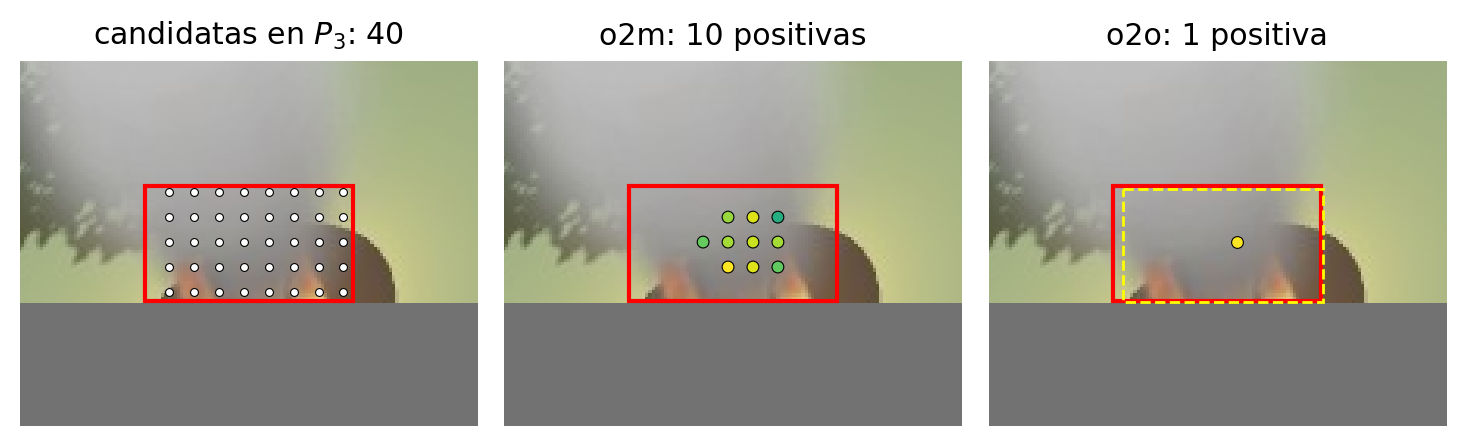
\includegraphics[width=\textwidth]{asignacion.png}
\caption{Asignación real en una imagen de validación con FuegoNet ya entrenada.
Izquierda: celdas candidatas de la caja de fuego (puntos grises) en la escala
$P_3$ (paso 8). Centro: las 10 celdas positivas de la cabeza o2m (color = métrica
$t$). Derecha: la única celda positiva de la o2o y, punteada, la caja que predice.}
\label{fig:asignacion}
\end{figure}

\section{STAL: que ningún foco se quede sin responsable}

Una celda es candidata solo si su \emph{centro} cae dentro de la caja. En la
escala más fina los centros están cada 8 píxeles. Un foco visto desde 60~m puede
medir $6\times5$ píxeles y caer entre cuatro centros sin contener ninguno. Esa
etiqueta queda sin celdas positivas, la red nunca aprende de ella y el error pasa
sin que se note.

STAL (\emph{Small-Target-Aware Label assignment}) resuelve esto. Si un lado de la
caja mide menos que el paso intermedio (16 píxeles), al buscar candidatas se
agranda a 16 píxeles alrededor de su centro. Solo se agranda para elegir
candidatas: el objetivo de la regresión sigue siendo la caja original.

\begin{lstlisting}[style=py]
    def _dentro(self, puntos, cajas):
        c = (cajas[..., :2] + cajas[..., 2:]) / 2
        wh = (cajas[..., 2:] - cajas[..., :2]).clamp(min=self.lado_min)      # STAL
        lt, rb = (c - wh / 2)[:, :, None], (c + wh / 2)[:, :, None]
        d = torch.cat((puntos - lt, rb - puntos), -1)                        # (B, M, A, 4)
        return d.amin(-1) > self.eps
\end{lstlisting}

\section{El código}

\paso{14} \textbf{Escribir \cod{AsignadorTAL}.}
Todo se hace con tensores de forma $(B, M, A)$: imágenes, etiquetas (rellenadas
con ceros hasta el máximo del lote) y celdas. No hay ciclos de Python sobre
celdas ni sobre etiquetas:

\begin{lstlisting}[style=py]
        dentro = self._dentro(puntos, cajas_gt) & valido.bool()              # (B, M, A)
        b, m, a = dentro.nonzero(as_tuple=True)
        iou[b, m, a] = ciou(cajas_gt[b, m], cajas_p[b, a]).clamp_(0)
        s[b, m, a] = prob[b, a, clases_gt[b, m, 0].long()]
        t = s.pow(self.alpha) * iou.pow(self.beta)
        idx = t.topk(self.topk, dim=-1).indices                               # (B, M, k)
        pos = torch.zeros_like(t, dtype=torch.int8).scatter_(-1, idx, 1)
        pos = pos * dentro * valido.to(torch.int8)
        varios = (pos.sum(1, keepdim=True) > 1).expand(-1, M, -1)            # conflictos
        mejor = torch.zeros_like(pos).scatter_(1, iou.argmax(1, keepdim=True), 1)
        pos = torch.where(varios, mejor, pos)
        if self.topk2 != self.topk:                                          # uno a uno
            idx2 = (t * pos).topk(self.topk2, dim=-1).indices
            pos = pos * torch.zeros_like(pos).scatter_(-1, idx2, 1)
\end{lstlisting}

\begin{aviso}
El asignador va decorado con \cod{@torch.no_grad()} y recibe las predicciones
con \cod{.detach()}. La asignación \emph{usa} la predicción para decidir, pero
no se deriva a través de esa decisión. Si se deriva, la red aprende a hacer
trampa con su propia asignación.
\end{aviso}

\begin{ejercicio}
En \cod{perdida.py} cambia \cod{lado_min} a 0 (STAL apagado), entrena 30 épocas y
compara el AP de fuego con el del modelo normal en las imágenes del mundo grande,
donde los focos se ven más pequeños.
\end{ejercicio}
